\documentclass[./dissertation.tex]{subfiles}
\begin{document}
    \chapter{Footnotes and Sidenotes}

    Dissertations will most likely include numerous side comments that are tangential to the main text. Generally, these are included in the document as footnotes or endnotes. With this template, you have the option to include them as \textit{sidenotes}, meaning they appear in the margin of your page rather than at the bottom.\footnote{Prior to 2020, this layout had not been used in a UGA dissertation. However, because of this {\LaTeX} template, the Graduate School and the format checkers approved the use of sidenotes specifically for us!} In this ``chapter'', we'll\footnote{I'll mention that this chapter was written primarily by Joey Stanley, so you'll know who's talking when I express my typographical opinions.} weigh the benefits and drawbacks of sidenotes and show you how you can toggle between them in your document.

    \section{Turning sidenotes on}

    The way to turn sidenotes on in this template is pretty straightforward. In the \texttt{dissertation.tex} file, you should find a command called \verb+sidenotetrue+. All you need to do is delete that line of code and type \verb+sidenotefalse+.

    \section{List of changes}

    If you do choose to turn the sidenotes on, be aware that it makes a couple other changes to your document. This section lists those changes.

    \subsection{Changes to the footnote command}

    The biggest change to your code is that the \verb+\footnote+ command has been recoded to now produce sidenotes. Specifically, the code that accomplishes this rewriting:
    \begin{verbatim}
      \renewcommand{\footnote}[1]{
          \sidenote{\RaggedRight\footnotesize #1}
      }
    \end{verbatim}
    This code essentially turns the \verb+\footnote+ function into a wrapper around the \verb+\sidenote+ function from the \texttt{sidenote} package. It also changes the default fully-justified behavior to ``ragged right.''\footnote{With a sidenote margin so small, it's basically impossible to have good-looking text if it's forced to align to the left and right margins. Using \texttt{RaggedRight} from the \texttt{ragged2e} package does a nice job at making a narrow column of text look nice.} Finally, it ensures the font size is footnote size.

    The reason for redefining \verb+\footnote+ rather than using \verb+\sidenote+ is becaue I wanted to make toggling between them as simple as possible. If you're three chapters into your dissertation and you decide you want to switch to the other layout, all you need to do is change one line of code. Had I required you to use \verb+\sidenote+, you would have to change the one command \textit{and} change all the \verb+\footnote+ commands to \verb+\sidenote+. I think doing it this way makes sense.

    \subsection{Changes to the page layout}

    If you have footnotes, the margins of your paper will be 1 inch on all sides, except for the bottom which is 1.25 inches.\footnote{This extra space is typo\-grahpically recommended to give the page a more balanced appearance.}. The body of the text is therefore centered, and there is no difference between even- and odd-sided pages.

    If you turn on the sidenotes though, we needed to make some extra room to accomodate them in the margin.\footnote{Ideally, we'd make the paper wider so that it's slightly more square. Most books that use sidenotes today are like that. It gives a little extra width to the margins so the sidenotes aren't so narrow. Alas, we are constrained by UGA and Print \& Copy in Tate since they can only bind specific paper sizes.} To accomplish this, we had to reformat the layout on the page.

    The biggest change is that the body of the text is now off-center. For odd-sided pages (meaning it would appear on the right side when you lay the book open), it's shifted towards the left and for even-sided pages (the left side of a two-page spread), it's shifted towards the right. In other words, the text is shifted towards the spine of the book. This leaves some room for the margins, which are towards the edges of the book. Here are the default dimensions:

    \begin{itemize}
      \item The top margin is 1 inch and the bottom margin is 1.25 inches.
      \item Starting from the edge of the page (on an odd-sided page), the outer margin is 0.75 inches. This is the distance from the page to the edge of your sidenotes.
      \item The sidenotes themselves are 1.5 inches wide.
      \item There is a one-eighth inch space between the sidenotes and the body text.
      \item The body text itself is 4.375 inches wide.
      \item The inner margin is 1 inch.
      \item There is an additional ``binding offset'' of a quarter inch added to the inside margin to accomodate for printing. This basically just means that the inside margin is 1.25 inches.
    \end{itemize}
    The outer margin has to be a little bit narrower than the typical 1 inch to give the body text enough room. Because footnotes are left-justified, this is not as noticeable on odd-sided pages, though on even-sided pages it's a little more obvious.



    \section{Details about how sidenote behavior}

    You should be aware of how the sidenotes behave, as they are implemented in this document. Sidenotes will be placed on the outer marin, but its their vertical positioning that may shift around.

    By default, sidenotes will start on the same line as the sidenote \textit{marker} (that is, the small superscripted number within the body of your text). If you use relatively few sidenotes, or if they're generally short, this is what you'll typicaly find.

    The question then is what happens if a sidenote runs up against the bottom of the page. Like if the sidenote marker is on the bottom line of a page and the sidenote itself is several lines long. As expected, the position of the sidenote itself will simply shift up so that it doens't spill into the bottom margin. Under the hood, while it is important that a sidenote be near its marker, is is \textit{more} important for the sidenote to not spill into the bottom margin, so that takes priority.

    Similarly, if you have multiple sidenotes that are near each other, the notes themselves will not overlap. They'll reposition themselves vertically along the margin so that they're as close to their markers as possible without overlapping with eaach other or with a top/bottom margin.

    For very long sidenotes,\footnote{Here is a very long sidenote so you can get a feel for what it looks like. Lorem ipsum dolor sit amet, consectetur adipisicing elit, sed do eiusmod tempor incididunt ut labore et dolore magna aliqua. Ut enim ad minim veniam, quis nostrud exercitation ullamco laboris nisi ut aliquip ex ea commodo consequat. Duis aute irure dolor in reprehenderit in voluptate velit esse cillum dolore eu fugiat nulla pariatur. Excepteur sint occaecat cupidatat non proident, sunt in culpa qui officia deserunt mollit anim id est laborum. Lorem ipsum dolor sit amet, consectetur adipisicing elit, sed do eiusmod tempor incididunt ut labore et dolore magna aliqua. Ut enim ad minim veniam, quis nostrud exercitation ullamco laboris nisi ut aliquip ex ea commodo consequat. Duis aute irure dolor in reprehenderit in voluptate velit esse cillum dolore eu fugiat nulla pariatur. Excepteur sint occaecat cupidatat non proident, sunt in culpa qui officia deserunt mollit anim id est laborum.} or for pages with many sidenotes such that they fill the margin completely, {\LaTeX} will do what it can to put it on the same page as the marker, but if it cannot, it will push it to the next page. For long footnotes, you may have seen them start on the correct page but spill over onto the next page---that behavior is unfortunately not possible with the current implementation of sidenotes in this template. For the most part this behavior is fine and readers typically are aware enough to look on the next page. However, be aware that should this next page be, say, the start of a new chapter, you'll get some unexpected sidenote placements.

    For sidenotes that are so long that they cannot fit on a single page, it will cause an error in {\LaTeX} and your document will not compile. If you typically have many very long sidenotes, it may be better to switch to a footnote layout.



    \section{Pros and Cons}

    With this information in mind, it's important to consider the pros and cons of using sidenotes.

    \subsection{Why I love sidenotes}

    There are lots of reasons why I love sidenotes. First off, since they were popularized by statisticiaon Edward Tufte\footnote{Note that there is a \texttt{tufte} package that creates sidenotes. Because we did not necessarily want to use the other changes that package makes to the document, we chose not to use it here.} in his books on data visualization, they've been used widely and are adopted by many typographers. The reason is simple: they just look nice. Rather than your eye having to dart to the bottom of the page and back, sidenotes are \textit{in situ}, and they do a nice job at making it easier for the reader to find them.

    In addition to making the sidenotes themselves easier to find and read, increasing the margin on one side makes the body text a little narrower. The typical 6.5 inch body text with 10- or 12-point font is a little too wide. The narrower layout, together with an appropriate line spacing, makes for a sophisticated layout that's easier to read than what you might be used to in a dissertation.

    Sidenotes are nice for putting some kinds of additional, non-textual information that are very vertical. It's possible to put a very narrow table, a very narrow image, or even a smaller image,\footnote{There's no need for an image to take up half a page when the information can be conveyed in tiny plot. Here's an actual image I included in my dissertation, showing the distribution of a particular variable. 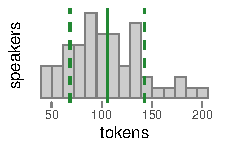
\includegraphics[width = 1.5in]{figures/tiny.pdf} It was handy to be able to have several of these little guys scattered around in the margins rather than taking up a huge chunk of the page.} icon, or plot in a sidenote.


    \subsection{Why you may not love sidenotes}

    First, as just mentioned, they're not ideal if you often use many long footnotes. If that's the case, you would probably be better off with the footnotes option.

    Another small issue relates to how this particular template is structured. You can work on each chapter and compile each chapter individually. However, because the command that reorganizes the layout on the page is on the \texttt{dissertation.tex} file, when you compile just a single chapter, you don't get the right layout. This can be kind of annoying.

    For certain things that may go in footnotes but are inherently wider, like formulas, computer code, extended quotations, data, numbered examples, or images, sidenotes are just too narrow. You're better off switching to footnotes if you make use of many of these. You may find a way to hack a one-off footnote if you need it for just one case.

    Finally, because I've redefined \verb+\footnote+ to do sidenotes, it's not possible to include both footnotes and sidenotes within your document. I have seen some books do this, but I'm not sure why you would need both. Fortunately, this is an easy fix: you would just remove the code in \texttt{dissertation.tex} that redefines footnotes, and now you're free to use \verb+\footnote+ and \verb+\sidenote+ independently of each other. This behavior has not been tested so you're on your own as far as debugging goes.



    \section{Hacking some less common cases}

    \subsection{Putting a plot in a sidenote}

    The code for the little plot I have in the sidenote above is this:
    \begin{verbatim}
      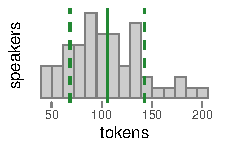
\includegraphics[width = 1.5in]{figures/tiny.pdf}
    \end{verbatim}
    Note that because these are so small, there is no figure number assigned to them and there's no caption. Consequently, they will not appear in the ``List of Figures'' in your frontmatter if you have one.

    \subsection{Others?}

    TODO.

\end{document}
